\documentclass[11pt]{article}
\usepackage[spanish]{babel}
\usepackage[utf8]{inputenc}
\usepackage{listings}
\usepackage{graphicx}
\graphicspath{{../Imagenes/}}

\usepackage[paper=portrait, pagesize]{typearea}
\usepackage{titlepic}

%%% Tablas
\usepackage{tabularx}
\usepackage{float}
\usepackage{adjustbox}
\usepackage{booktabs}
\usepackage{multirow}
\renewcommand{\arraystretch}{1.7}

\begin{document}

\begin{titlepage}
\centering
\vspace{4.5cm}
{\scshape\LARGE Descripción inicial del sistema. Modelado de usuarios y escenarios \par}
\vspace{1.5cm}


\includegraphics[width=16cm] {Logo}

\vspace{3cm}
{\scshape\large \par}
\vspace{1cm}

{Miguel Albertí Pons\\
Sofía Almeida Bruno\\
Pedro Manuel Flores Crespo\\
María Victoria Granados Pozo\\
Lidia Martín Chica
\par}

\end{titlepage}


\newpage

\section{Personajes}
%%TABLA JAVI
\begin{table}[H]
  \centering
  \begin{tabular}{p{0.2\linewidth}|p{0.3\linewidth}p{0.475\linewidth}}
    \toprule
    \textbf{Nombre} & Javier Martín Parra &\multirow{4}{*}{\begin{minipage}{1.\textwidth}
\includegraphics[width=0.2\textwidth, height=30mm]{Javier}\end{minipage}}\\
    \textbf{Edad} & 23 & \\
    \textbf{Sexo} & Hombre & \\
    \textbf{Educación} & Graduado en Historia & \\
    \bottomrule
  \end{tabular}

  \begin{tabular}{l}
    \textbf{Contexto de uso} 
  \end{tabular}
  
  \begin{tabular}{p{0.2\linewidth}|p{0.8\linewidth}}
    \toprule
    \textbf{Cuándo} & El domingo, ya que es su día libre en la preparación de las oposiciones\\
    \textbf{Dónde}  & En su casa\\
    \textbf{Tipo de ordenador} & En este caso, utiliza su dispositivo móvil\\
    \bottomrule
  \end{tabular}

  \begin{tabular}{l}
    \textbf{Misión} 
  \end{tabular}
  
  \begin{tabular}{p{0.2\linewidth}|p{0.8\linewidth}}
    \toprule
    \textbf{Objetivo} & Organizar un viaje a Turquía\\
    \textbf{Expectativas}  & Espera aprovechar las experiencias de otros usuarios para que su viaje sea inolvidable \\
    \bottomrule
  \end{tabular}

  \begin{tabular}{l}
    \textbf{Motivación} 
  \end{tabular}

  \begin{tabular}{p{0.2\linewidth}|p{0.8\linewidth}}
    \toprule
    \textbf{Urgencia} & Como quiere realizar el viaje cuando termine las oposiciones, no tiene mucha prisa\\
    \textbf{Deseo}  & Le gustaría hacer este viaje para aprender más sobre el imperio bizantino \\
    \bottomrule
  \end{tabular}

  \begin{tabular}{p{1.028\linewidth}}
    \textbf{Actitud hacia la tecnología}\\
    \midrule
    Ha nacido en la época digital y utiliza con total confianza todo tipo de dispositivos y aplicaciones, tanto nuevas como ya conocidas
  \end{tabular}
\end{table}

\newpage

%%TABLA PEDRO
\begin{table}[H]
  \centering
  \begin{tabular}{p{0.2\linewidth}|p{0.3\linewidth}p{0.475\linewidth}}
    \toprule
    \textbf{Nombre} & Pedro Barranco Sánchez &\multirow{4}{*}{\begin{minipage}{1.\textwidth}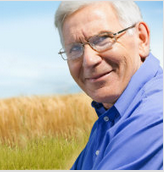
\includegraphics[width=0.2\textwidth, height=30mm]{Pedro}\end{minipage}}\\
    \textbf{Edad} & 73 & \\
    \textbf{Sexo} & Hombre & \\
    \textbf{Educación} & Jubilado & \\
    \bottomrule
  \end{tabular}

  \begin{tabular}{l}
    \textbf{Contexto de uso} 
  \end{tabular}
  
  \begin{tabular}{p{0.2\linewidth}|p{0.8\linewidth}}
    \toprule
    \textbf{Cuándo} & Casi todos los días después de comer\\
    \textbf{Dónde}  & En su casa\\
    \textbf{Tipo de ordenador} & Usa una tablet\\
    \bottomrule
  \end{tabular}

  \begin{tabular}{l}
    \textbf{Misión} 
  \end{tabular}
  
  \begin{tabular}{p{0.2\linewidth}|p{0.8\linewidth}}
    \toprule
    \textbf{Objetivo} & Buscar un regalo para su mujer por el aniversario\\
    \textbf{Expectativas}  & Encontrar un evento cultural en su ciudad, y que llegue el transporte público \\
    \bottomrule
  \end{tabular}

  \begin{tabular}{l}
    \textbf{Motivación} 
  \end{tabular}

  \begin{tabular}{p{0.2\linewidth}|p{0.8\linewidth}}
    \toprule
    \textbf{Urgencia} & No mucha, ya que buscará eventos para todo el mes\\
    \textbf{Deseo}  & Pasar una noche diferente con su mujer \\
    \bottomrule
  \end{tabular}

  \begin{tabular}{p{1.028\linewidth}}
    \textbf{Actitud hacia la tecnología}\\
    \midrule
    No entiende la tablet muy bien, y por eso se pone nervioso cuando no sabe hacer algo
  \end{tabular}
\end{table}

%%TABLA ANA
\begin{table}[H]
  \centering
  \begin{tabular}{p{0.2\linewidth}|p{0.3\linewidth}p{0.475\linewidth}}
    \toprule
    \textbf{Nombre} & Ana García Blanco &\multirow{4}{*}{\begin{minipage}{1.\textwidth}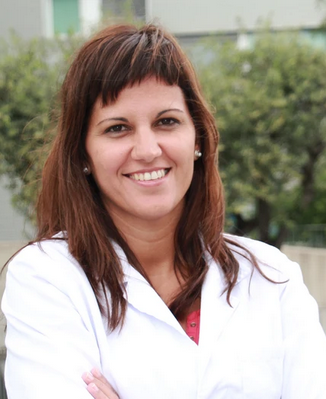
\includegraphics[width=0.2\textwidth, height=30mm]{Ana}\end{minipage}}\\
    \textbf{Edad} & 38 & \\
    \textbf{Sexo} & Mujer & \\
    \textbf{Educación} & Cirujana & \\
    \bottomrule
  \end{tabular}

  \begin{tabular}{l}
    \textbf{Contexto de uso} 
  \end{tabular}
  
  \begin{tabular}{p{0.2\linewidth}|p{0.8\linewidth}}
    \toprule
    \textbf{Cuándo} & En viernes en la guardia del hospital\\
    \textbf{Dónde}  & En el hospital\\
    \textbf{Tipo de ordenador} & Móvil personal\\
    \bottomrule
  \end{tabular}

  \begin{tabular}{l}
    \textbf{Misión} 
  \end{tabular}
  
  \begin{tabular}{p{0.2\linewidth}|p{0.8\linewidth}}
    \toprule
    \textbf{Objetivo} & Organizar una actividad familiar para el domingo\\
    \textbf{Expectativas}  & Realizar la actividad cerca de su pueblo y que no tenga un coste elevado \\
    \bottomrule
  \end{tabular}

  \begin{tabular}{l}
    \textbf{Motivación} 
  \end{tabular}

  \begin{tabular}{p{0.2\linewidth}|p{0.8\linewidth}}
    \toprule
    \textbf{Urgencia} & Máxima, porque quiere realizar la actividad este fin de semana\\
    \textbf{Deseo}  & Disfrutar de un bonito día en familia y no tener que dedicar mucho tiempo a encontrar la actividad\\
    \bottomrule
  \end{tabular}

  \begin{tabular}{p{1.028\linewidth}}
    \textbf{Actitud hacia la tecnología}\\
    \midrule
    Tiene manejo de las tecnologías, pero aún así es precavida.  
  \end{tabular}
\end{table}

%%TABLA MARÍA
\begin{table}[H]
	\centering
	\begin{tabular}{p{0.2\linewidth}|p{0.3\linewidth}p{0.475\linewidth}}
		\toprule
		\textbf{Nombre} & María Delgado Lucena &\multirow{4}{*}{\begin{minipage}{1.\textwidth}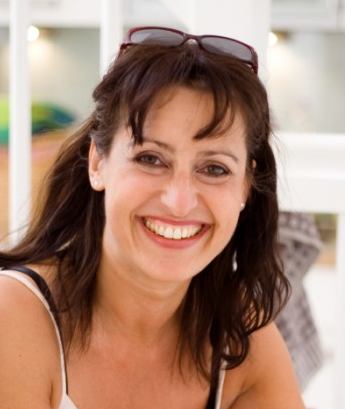
\includegraphics[width=0.2\textwidth, height=30mm]{Maria}\end{minipage}}\\
		\textbf{Edad} & 45 & \\
		\textbf{Sexo} & Mujer & \\
		\textbf{Educación} & Ama de casa & \\
		\bottomrule
	\end{tabular}
	
	\begin{tabular}{l}
		\textbf{Contexto de uso} 
	\end{tabular}
	
	\begin{tabular}{p{0.2\linewidth}|p{0.8\linewidth}}
		\toprule
		\textbf{Cuándo} & Por la tarde, después del almuerzo \\
		\textbf{Dónde}  & En casa\\
		\textbf{Tipo de ordenador} & Móvil personal\\
		\bottomrule
	\end{tabular}
	
	\begin{tabular}{l}
		\textbf{Misión} 
	\end{tabular}
	
	\begin{tabular}{p{0.2\linewidth}|p{0.8\linewidth}}
		\toprule
		\textbf{Objetivo} & Organizar una actividad para un grupo numeroso\\
		\textbf{Expectativas}  & Encontrar alguna ruta o paquete por España que incluya actividades que se puedan hacer en grupo \\
		\bottomrule
	\end{tabular}
	
	\begin{tabular}{l}
		\textbf{Motivación} 
	\end{tabular}
	
	\begin{tabular}{p{0.2\linewidth}|p{0.8\linewidth}}
		\toprule
		\textbf{Urgencia} & Normal, tiene tiempo para planificar el viaje\\
		\textbf{Deseo}  & El viaje lo organiza para la asociación de vecinos del barrio. Han acordado conocer más en este viaje acerca de la España rural para que sea más relajado y alejado del estrés de la ciudad\\
		\bottomrule
	\end{tabular}
	
	\begin{tabular}{p{1.028\linewidth}}
		\textbf{Actitud hacia la tecnología}\\
		\midrule
		No está acostumbrada a utilizar la tecnología pero no es reticente a utilizarla
	\end{tabular}
\end{table}


\newpage
\section{Escenarios}

%ESCENARIO 1
\begin{table}[H]
  \centering
  \begin{tabular}{p{0.2\linewidth}|p{0.3\linewidth}p{0.475\linewidth}}
    \toprule
    \textbf{Nombre de la persona} & Ana García Blanco &\multirow{2}{*}{\begin{minipage}{1.\textwidth}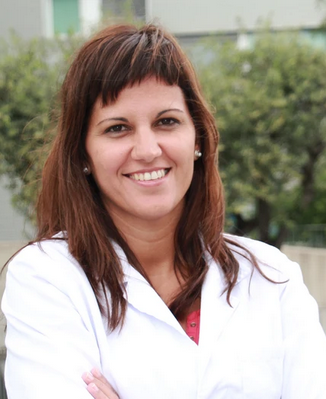
\includegraphics[width=0.2\textwidth, height=25mm]{Ana}\end{minipage}}\\
    \textbf{Objetivo persona} & Organizar una actividad familiar para el domingo & \\
    \bottomrule
  \end{tabular}

\begin{tabular}{p{1.028\linewidth}}
  \textbf{Escenario}\\
  \midrule  
  Ana quiere realizar una actividad el domingo cerca de su pueblo natal. El viernes al entrar en el trabajo se ha puesto con la aplicación MakeATravel para buscar una plan que cumpla con sus exigencias.
Necesita una actividad adaptada para niños donde pueda llevar a su hija pequeña y pasar un gran día en familia.

Gracias a los filtros de la aplicación, puede ver las distintas excursiones que estarán disponibles para ese día, además de información como hora de inicio, precio, la ruta para llegar y las opiniones de otros usuarios que ya hayan estado. Este último factor hará que, finalmente, elija una excursión por Sierra Nevada.

\end{tabular}
\end{table}


%ESCENARIO 2
\begin{table}[H]
  \centering
  \begin{tabular}{p{0.2\linewidth}|p{0.3\linewidth}p{0.475\linewidth}}
    \toprule
    \textbf{Nombre de la persona} & Ana García Blanco &\multirow{2}{*}{\begin{minipage}{1.\textwidth}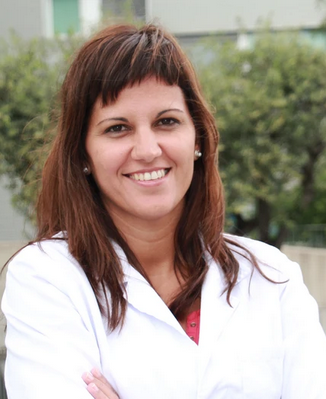
\includegraphics[width=0.2\textwidth, height=25mm]{Ana}\end{minipage}}\\
    \textbf{Objetivo persona} & Comentar y valorar una actividad que ha realizado & \\
    \bottomrule
  \end{tabular}

\begin{tabular}{p{1.028\linewidth}}
  \textbf{Escenario}\\
  \midrule
  Ana llega a su casa el domingo por la noche cansada tras finalizar la excursión a Sierra Nevada que había organizo con tanta ilusión. Accede a la aplicación para dar reflejar su opinión sobre la misma. Primero, escribe un comentario quejándose sobre la información que se aporta en la actividad, ya que indicaba que la excursión duraría dos horas y han sido tres. Además, no era apta para su hija ya que era una ruta muy complicada para niños debido a que la zona era demasiado escarpada. Finalmente, valora la actividad con la puntuación más baja posible. 
\end{tabular}
\end{table}


%ESCENARIO 3
\begin{table}[H]
  \centering
  \begin{tabular}{p{0.2\linewidth}|p{0.3\linewidth}p{0.475\linewidth}}
    \toprule
    \textbf{Nombre de la persona} & Pedro Barranco Sánchez &\multirow{2}{*}{\begin{minipage}{1.\textwidth}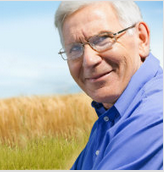
\includegraphics[width=0.2\textwidth, height=25mm]{Pedro}\end{minipage}}\\
    \textbf{Objetivo persona} & Identificarse en la aplicación & \\
    \bottomrule
  \end{tabular}

\begin{tabular}{p{1.028\linewidth}}
  \textbf{Escenario}\\
  \midrule
  Pedro está buscando un regalo de aniversario para su mujer. Después de comer, coge la tablet y abre la aplicación MakeATravel para buscar algún evento cultural, como por ejemplo un teatro o una ópera que haya en su ciudad. Su nieto, Jaime, fue el que le habló de la aplicación. Jaime desde su móvil registró a su abuelo ya que Pedro no sabía cómo rellenar el formulario que le aparecía. Ahora, al abrir la aplicación se encuentra una pantalla de identificación. No sabe qué hacer, no es la pantalla de actividades que su nieto le había enseñado a manejar. Decide llamar a Jaime por teléfono preguntándole qué hacer. Su nieto muy amablemente le responde ya que es consciente de que su abuelo y la tecnología no se llevan muy bien. Le recuerda que le escribió estos datos en un papel que guardó en el cajón del escritorio. Con las indicaciones de su nieto Pedro es capaz de introducir los datos necesarios para identificarse y empezar a usar la aplicación.

\end{tabular}
\end{table}

%ESCENARIO 3
\begin{table}[H]
	\centering
	\begin{tabular}{p{0.2\linewidth}|p{0.3\linewidth}p{0.475\linewidth}}
		\toprule
		\textbf{Nombre de la persona} & Pedro Barranco Sánchez &\multirow{2}{*}{\begin{minipage}{1.\textwidth}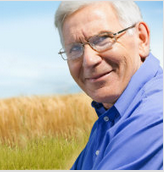
\includegraphics[width=0.2\textwidth, height=25mm]{Pedro}\end{minipage}}\\
		\textbf{Objetivo persona} & Encontrar una actividad para realizar con su mujer & \\
		\bottomrule
	\end{tabular}
	
	\begin{tabular}{p{1.028\linewidth}}
		\textbf{Escenario}\\
		\midrule
		Pedro ya está identificado y listo para buscar la actividad que desea. En el papel que su nieto le había escrito, también había algunas indicaciones sobre cómo encontrar la categoría que quiere, eventos culturales.Tras varios días de búsqueda en el solo aparecen teatros infantiles encuentra una obra teatral que se realizará a finales de mes. En ella la compañía ofrecerá una versión moderna y actual del clásico "La vida es sueño" de Calderón de la Barca. Accede a la información para ver la página oficial del teatro y poder comprar las entradas.
		
	\end{tabular}
\end{table}


%ESCENARIO 4
\begin{table}[H]
  \centering
  \begin{tabular}{p{0.2\linewidth}|p{0.3\linewidth}p{0.475\linewidth}}
    \toprule
    \textbf{Nombre de la persona} & María Delgado Lucena &\multirow{2}{*}{\begin{minipage}{1.\textwidth}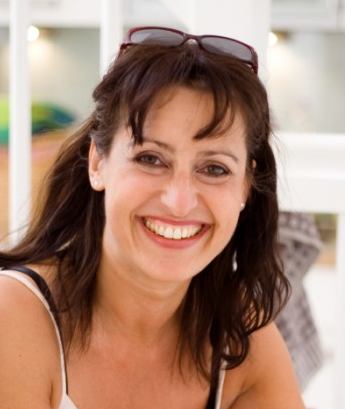
\includegraphics[width=0.2\textwidth, height=25mm]{Maria}\end{minipage}}\\
    \textbf{Objetivo persona} & Encontrar una actividad en grupo & \\
    \bottomrule
  \end{tabular}

\begin{tabular}{p{1.028\linewidth}}
  \textbf{Escenario}\\
  \midrule
	Tras el almuerzo, María se sienta en el sofá de su casa. El día anterior, tuvieron reunión en la asociación de vecinos del barrio. El tema a tratar era el viaje anual que realizan. Tras debatir, decidieron que el de este año sería un viaje por pueblos de toda España ya que el anterior fue a una ciudad demasiado concurrida que contrastaba con la tranquilidad que buscaban. Como la persona que se había encargado de organizarlos hasta el momento se había mudado, María se ofreció para organizarlo, aunque nunca antes lo había hecho.
	
	Por ello, abre al aplicación MakeATravel en su móvil. Va pasando progresivamente por las distintas categorías que ofrece la aplicación ya que no está muy segura de dónde buscar lo que desea. En un momento dado, encuentra una ruta por pueblos en el norte del país. Apunta la información más relevante que aporta la aplicación para contarla en la siguiente reunión. 
\end{tabular}
\end{table}


%ESCENARIO 5
\begin{table}[H]
  \centering
  \begin{tabular}{p{0.2\linewidth}|p{0.3\linewidth}p{0.475\linewidth}}
    \toprule
    \textbf{Nombre de la persona} & María Delgado Lucena &\multirow{2}{*}{\begin{minipage}{1.\textwidth}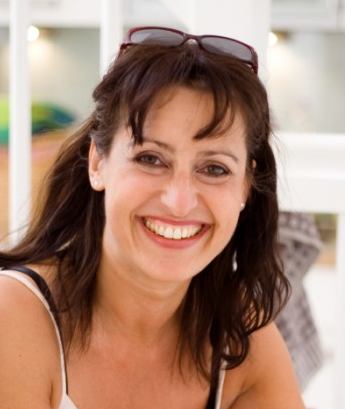
\includegraphics[width=0.2\textwidth, height=25mm]{Maria}\end{minipage}}\\
    \textbf{Objetivo persona} & Personalizar la ruta & \\
    \bottomrule
  \end{tabular}

\begin{tabular}{p{1.028\linewidth}}
  \textbf{Escenario}\\
  \midrule
  María está en la reunión junto con sus vecinos explicándoles lo que ha encontrado en la aplicación. Expone la información que había apuntado previamente. Al acabar, muchos vecinos le comunican que tienen dudas acerca de los datos que ha aportado, sobre todo acerca de la posibilidad de ir un grupo numeroso de personas. María vuelve a meterse en la aplicación pero no sabe cómo recuperar la ruta que había encontrado antes. Por ello, intenta recordar y repetir el proceso que había realizado. Finalmente la encuentra pero como no está toda la información que desean deciden leer los comentarios. Tienen suerte y encuentran uno donde un usuario advierte que en una de las actividades tuvieron ciertos problemas por ir en grupo. Uno de los vecinos propone realizar la ruta pero eliminando esa parada por lo María, desde la aplicación, accede a la ruta y la modifica eliminándola.  
\end{tabular}
\end{table}


%ESCENARIO 6
\begin{table}[H]
  \centering
  \begin{tabular}{p{0.2\linewidth}|p{0.3\linewidth}p{0.475\linewidth}}
    \toprule
    \textbf{Nombre de la persona} & Javier Martín Parra &\multirow{2}{*}{\begin{minipage}{1.\textwidth}
\includegraphics[width=0.2\textwidth, height=25mm]{Javier}\end{minipage}}\\
    \textbf{Objetivo persona} & Registrarse en la aplicación & \\
    \bottomrule
  \end{tabular}

\begin{tabular}{p{1.028\linewidth}}
  \textbf{Escenario}\\
  \midrule
  
  Tras una dura semana de estudio, Javier se dispone a encontrar el viaje perfecto a Turquía. Como estudió Historia espera que, además de ser un viaje lucrativo, también sea un viaje cultural en el que pueda aprender más sobre el imperio bizantino. Aunque el viaje lo realizará en unos meses, al terminar las oposiciones, quiere tenerlo preparado antes de empezar con los exámenes y no dedicarle mucho tiempo a su organización. Su amigo José Luis le ha estado hablando muy positivamente acerca de una nueva aplicación que ha estado usando para planificas sus viajes. Tras descargarla en su teléfono móvil, la abre y aparece un formulario de registro. Al estar familiarizado con este tipo de trámites, no tiene problema en rellenarlo y empezar a usar la aplicación de manera inmediata. 
\end{tabular}
\end{table}


%ESCENARIO 7
\begin{table}[H]
  \centering
  \begin{tabular}{p{0.2\linewidth}|p{0.3\linewidth}p{0.475\linewidth}}
    \toprule
    \textbf{Nombre de la persona} & Javier Martín Parra &\multirow{2}{*}{\begin{minipage}{1.\textwidth}
\includegraphics[width=0.2\textwidth, height=25mm]{Javier}\end{minipage}}\\
    \textbf{Objetivo persona} & Ofertar actividades & \\
    \bottomrule
  \end{tabular}

\begin{tabular}{p{1.028\linewidth}}
  \textbf{Escenario}\\
  \midrule
  Después de realizar el viaje a Turquía, Javier está muy contento de haber utilizado la aplicación MakeATravel. Se dispone a entrar de nuevo en la misma para ofertar nuevas actividades que realizó durante su viaje que le gustaron mucho pero que no estaban registradas. Las descubrió gracias a que se las recomendaron en la recepción del hotel en Turquía. Como le parecieron interesantes ha decidido ofertarlas para que puedan verlas y seleccionarlas otros usuarios con intereses similares. Al estar registrado e identificado, solo tiene que acceder a la sección de ofertar y completar la información que le pide la aplicación sobre cada una de las actividades.
\end{tabular}
\end{table}




\end{document}
